% !TeX root = ../main.tex
% Add the above to each chapter to make compiling the PDF easier in some editors.

\chapter{Concept and Integration}\label{chapter:integration}

With the assistance of the CMC framework, achieving mutual attestation across various confidential computing technologies becomes more accessible. The primary objective of enhancing this framework is the analysis of the different attestation concepts inherent to each technology and their integration into the overarching framework. This chapter will focus on the design considerations necessary for incorporating Intel SGX support into the framework. It will delve into the communication flow between an enclave and the CMC, outline the specific structure of an attestation report and identify additional data, that is required for a successful verification.

\section{Designing a mutual attestation concept for Intel SGX enclaves}
The core concept of the CMC is based on the so-called Mutual Attestation, i.e. the mutual verification of two or more TEEs. These TEEs can be of different types, e.g. a AMD SEV VM and an Intel SGX enclave, and run typically run on two separate systems.
The CMC Daemon provides endpoints for generation or verification of attestation reports as as well as the setup of an attested TLS channel. Certificates and other metadata is provided by a dedicated server running on the attesting platform.
While this approach works well for secure VM environments and TPMs, it is not suitable for SGX enclaves. By design however, only one process can run within an enclave. This means, the CMCD and the estserver cannot run within the trusted environment and therefore have to be executed in untrusted memory. 

Nevertheless, this procedure still works since the enclave can make corresponding ECALLs and OCALLs to read and write data from untrusted memory and to call functions outside the enclave. However, loading data from untrusted memory into the enclave always poses a certain security risk, as this could potentially be tampered with.  
In this case, however, all components (the quote, certificate chains and other metadata) are signed and thus integrity-protected, which means manipulation of the data would be detected in the verification process. Furthermore, protection against replay attacks is mitigated, by including a nonce provided by the client in the attestation report. 

\begin{figure}
	\begin{center} 
		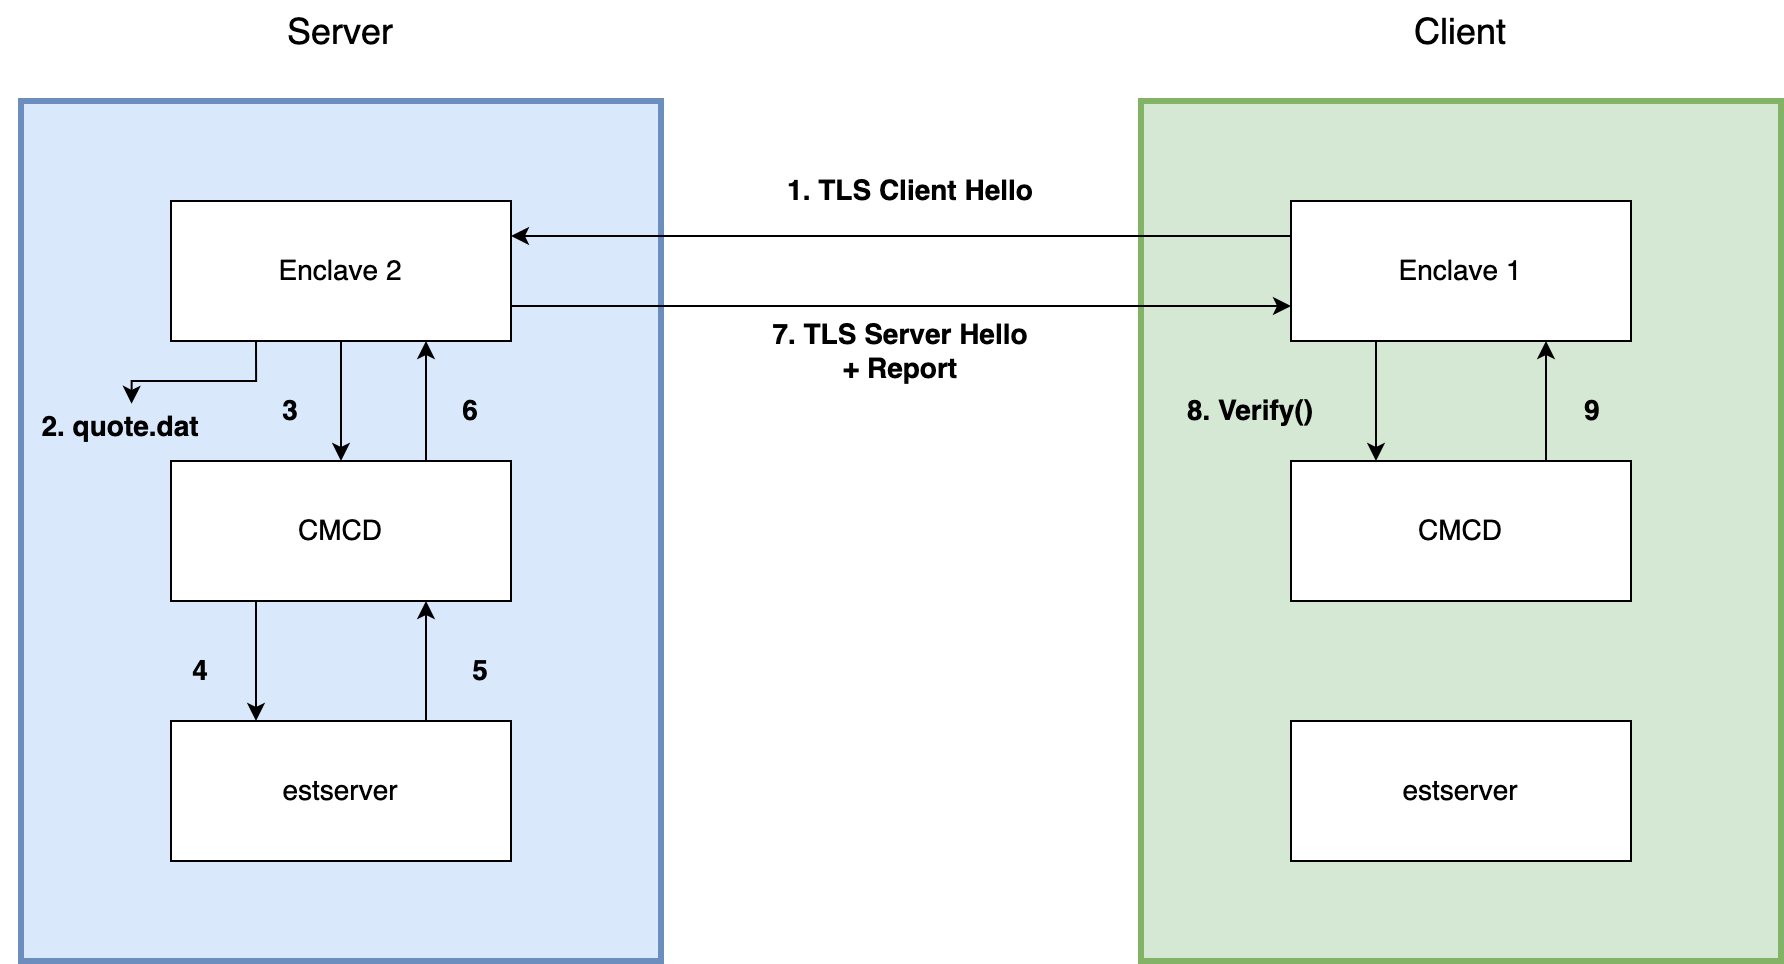
\includegraphics[width=1.0\linewidth]{figures/cmc-sgx-concept.drawio.png}
	\end{center}
	\caption{First SGX attestation concept}
	\label{sgx-concept-01}
\end{figure}

Following this concept, the attestation control flow of the CMC can be structured in the following way (depicted in figure \ref{sgx-concept-01}):  
\begin{enumerate}
	\item The client initiates a TLS connection to the enclave and requests an attestation report.
	\item The enclave generates an attestation report inside the enclave by utilizing the Intel SGX library and includes the hash of the TLS master public key inside the report. This report is converted by the QE into a signed Quote and stored in the filesystem.
	\item Then the enclave calls the report generation service of the CMCD, e.g. by making an OCALL to the specific gRPC endpoint.
	\item The CMCD reads the signed quote file from the filesystem and combines it with signed metadata retrieved from the estserver into a CMC report structure.
	\item This data is sent back to the enclave application and then loaded into the enclave via an ECALL.
	\item The enclave then finally forwards the report as well as the chosen cipher-mode and public key certificate to the client, which can now verify the attestation report by making corresponding calls to the gRPC verification endpoint of the CMCD running on his side.
\end{enumerate}

After the report has been successfully validated, the client can securely communicate with the TEE over an attested TLS channel. To complete the mutual attestation, the server also has to request and validate an attestation report from the client TEE. 

Even though this architecture implements the current CMC concept, it is not ideal.
First of all the context switches in and out of the enclave introduce additional overhead. In a production environment, with potentially hundrets or thousands of attestation requests per second, this overhead becomes significant. Moreover, in and out of the enclave with the E-/OCALLs, in a big production environment with possibly many incoming attestation requests per second, the overhead of switching in and out of the enclave is not neglectable.

Moreover, loading and parsing data from untrusted memory into an enclave can introduce possibly malicious code, which could lead to undefined behavior or even buffer overflow attacks. The enclave therefore needs to be hardened against such attacks, which requires an in-depth security analysis, depending on how the enclave handles the incoming data. Another security risk poses the transport of the attestation report between the enclave and the cmcd. In this example (figure \ref{sgx-concept-01}) the quote remains unencrypted while resting on the file system and the cmc report is transported over an unencrypted TCP connection between the cmcd and the enclave. Although the attestation report doesn’t contain highly sensitive data, the information about TCB Level, measurements, enclave attributes, and other metadata can possibly be valuable for an attacker. 

As can be seen, the core problem is the communication with untrusted components. To address this issue the entire attestation report generation must happen inside the enclave. This can be achieved by using the cmc not as service, but as a program library.


\begin{figure}
	\begin{center} 
		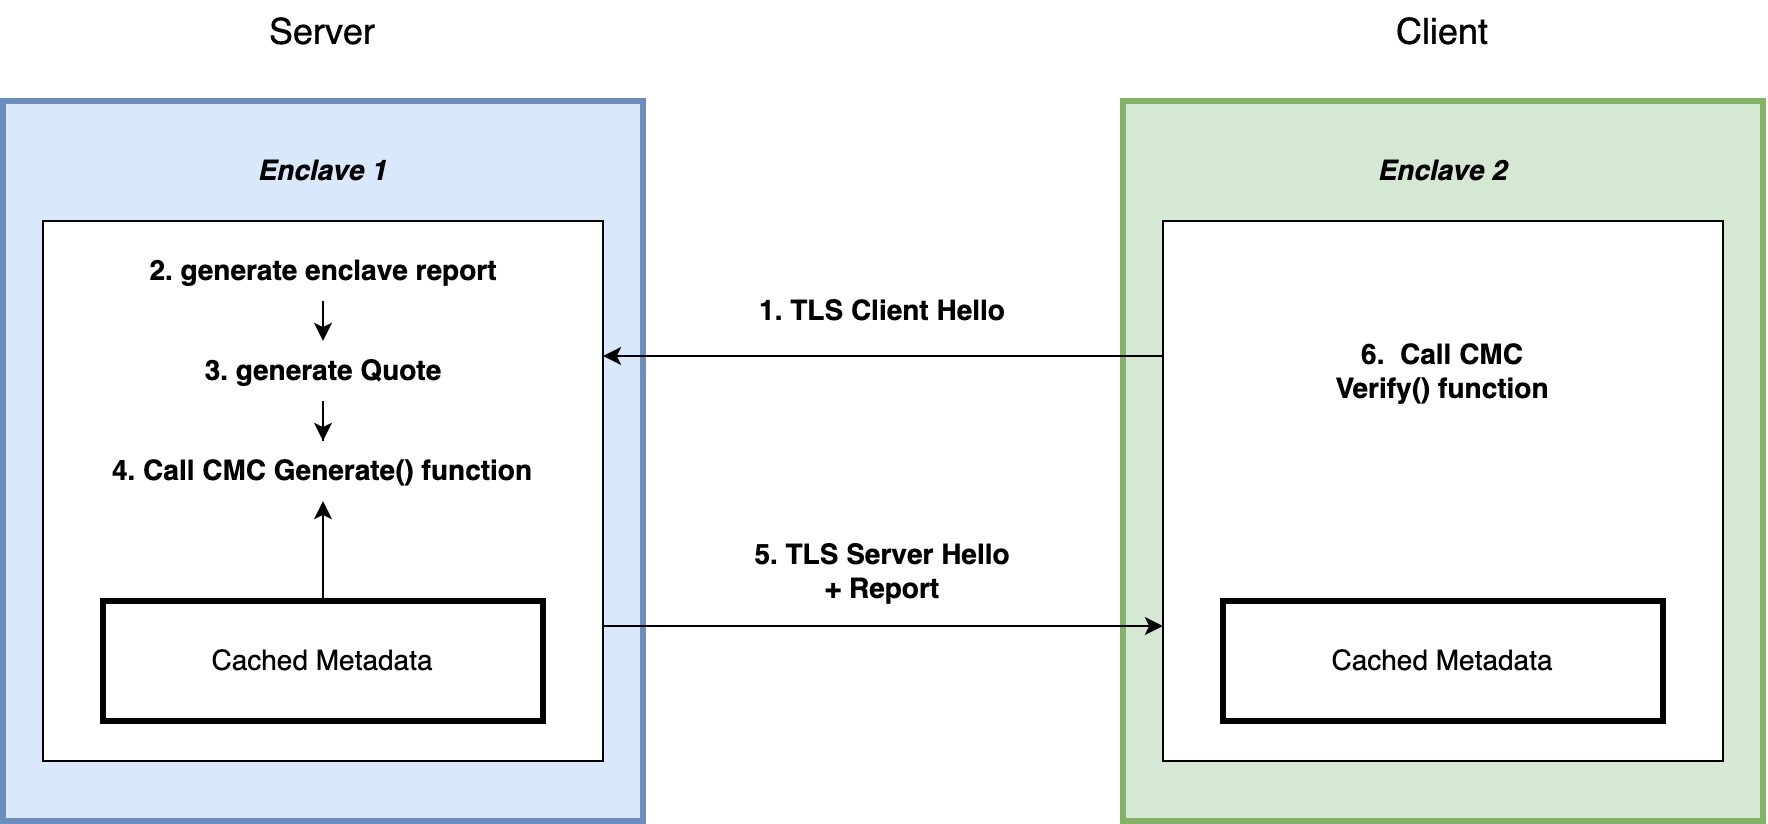
\includegraphics[width=1.0\linewidth]{figures/cmc-sgx-concept2.drawio.png}
	\end{center}
	\caption{Improved SGX Attestation concept} 
	\label{sgx-concept-02}
\end{figure}
Based on this principle, the attestation flow has to be adapted (see figure \ref{sgx-concept-02}): 
Assuming again both sides are running within one enclave, first the client sends a request to the server to initiate the TLS connection. In response, the server first creates an enclave report, then turns this report into a quote, by calling the Intel library quote generation function (3). This quote is then passed to the report generation function of the cmc library (4), which wraps it into the cmc attestation report structure, combined with the corresponding metadata. To avoid any unnecessary and potential dangerous OCALLs, the metadata is cached inside the enclave as well. 
After the report has been generated it is finally sent back to the client in the TLS response (5). In turn, the client calls the appropriate quote verification function of the cmc library and decides, based on the result, whether the enclave is trustworthy or not. 
Again, to complete the mutual attestation the server also has to request and verify a report from the client.

This approach fixes most of the previous concerns. However, another problem poses the caching of metadata inside the enclave. While most of the data remains stable over time, certain information changes periodically, e.g. the PCK certificate and CRLs. By design, all data inside the enclave page cache must already be included at compile time. Instead of recompiling the entire enclave only for a few values, the enclave can use OCALLs to request updated information from the PCCS. Once again, this provides an inside attacker according to the Threat Model with a potential point of attack. (More on this in Chapter \ref{chapter:evaluation} - Security Analysis).

\section{Analyzing the SGX Report structure and identifying metadata}

An SGX Quote, i.e. the signed remote attestation report, is basically structured as follows: It consists of a 48-byte header, a 384-byte report body and a quote signature data structure of variable size. (table \ref{quote-overview-table}).

The header contains information about the report, such as the version number, the attestation key type, TEE type (i.e. SGX or TDX), secure version numbers, etc. 

The report body contains the enclaves's attestation report. It holds values such as the CPU SVN, an enclave measurement hash, a hash of the enclave signing key and even 64 byte of custom data supplied by the enclave owner (table \ref{quote-body-table}).

The quote signature data structure (table \ref{quote-signature-table}) comprises essential components required for cryptographic validation. Most importantly it consists of the public key of the ECDSA Attestation key, generated by the Quoting Enclave (QE) and the ECDSA signature of the enclave report. Furthermore it contains the attestation report from the QE, a QE Authentication Data field, which provides supplementary information about the Quoting Enclave and lastly a QE Certification Data field with additional information required for the signature validation. \cite{dcap_library_doc}

In order to verify such an SGX Quote, the DCAP Library's Quote Verification function requires additional data. The DCAP Library calls this \textit{Quote collateral} - A single structure, including values such as CRLs, a TCB Info structure, a QE Identity structure and certificate chains.\ref{quote-collateral-table} - The PCCS database, contains all of this information in separate tables. According to the DCAP Quote verification library, this datastructure can either be passed to the verification function directly or it autonomously retrieved by the function itself. Noted, that this is only possible, if the PCCS is running on the same platform as the verifier. 
Because this typically not the case, the cmc has to combine this information inside the overarching report structure. 

\section{Analyzing the CMC Report structure}

\begin{figure}
	\begin{center} 
		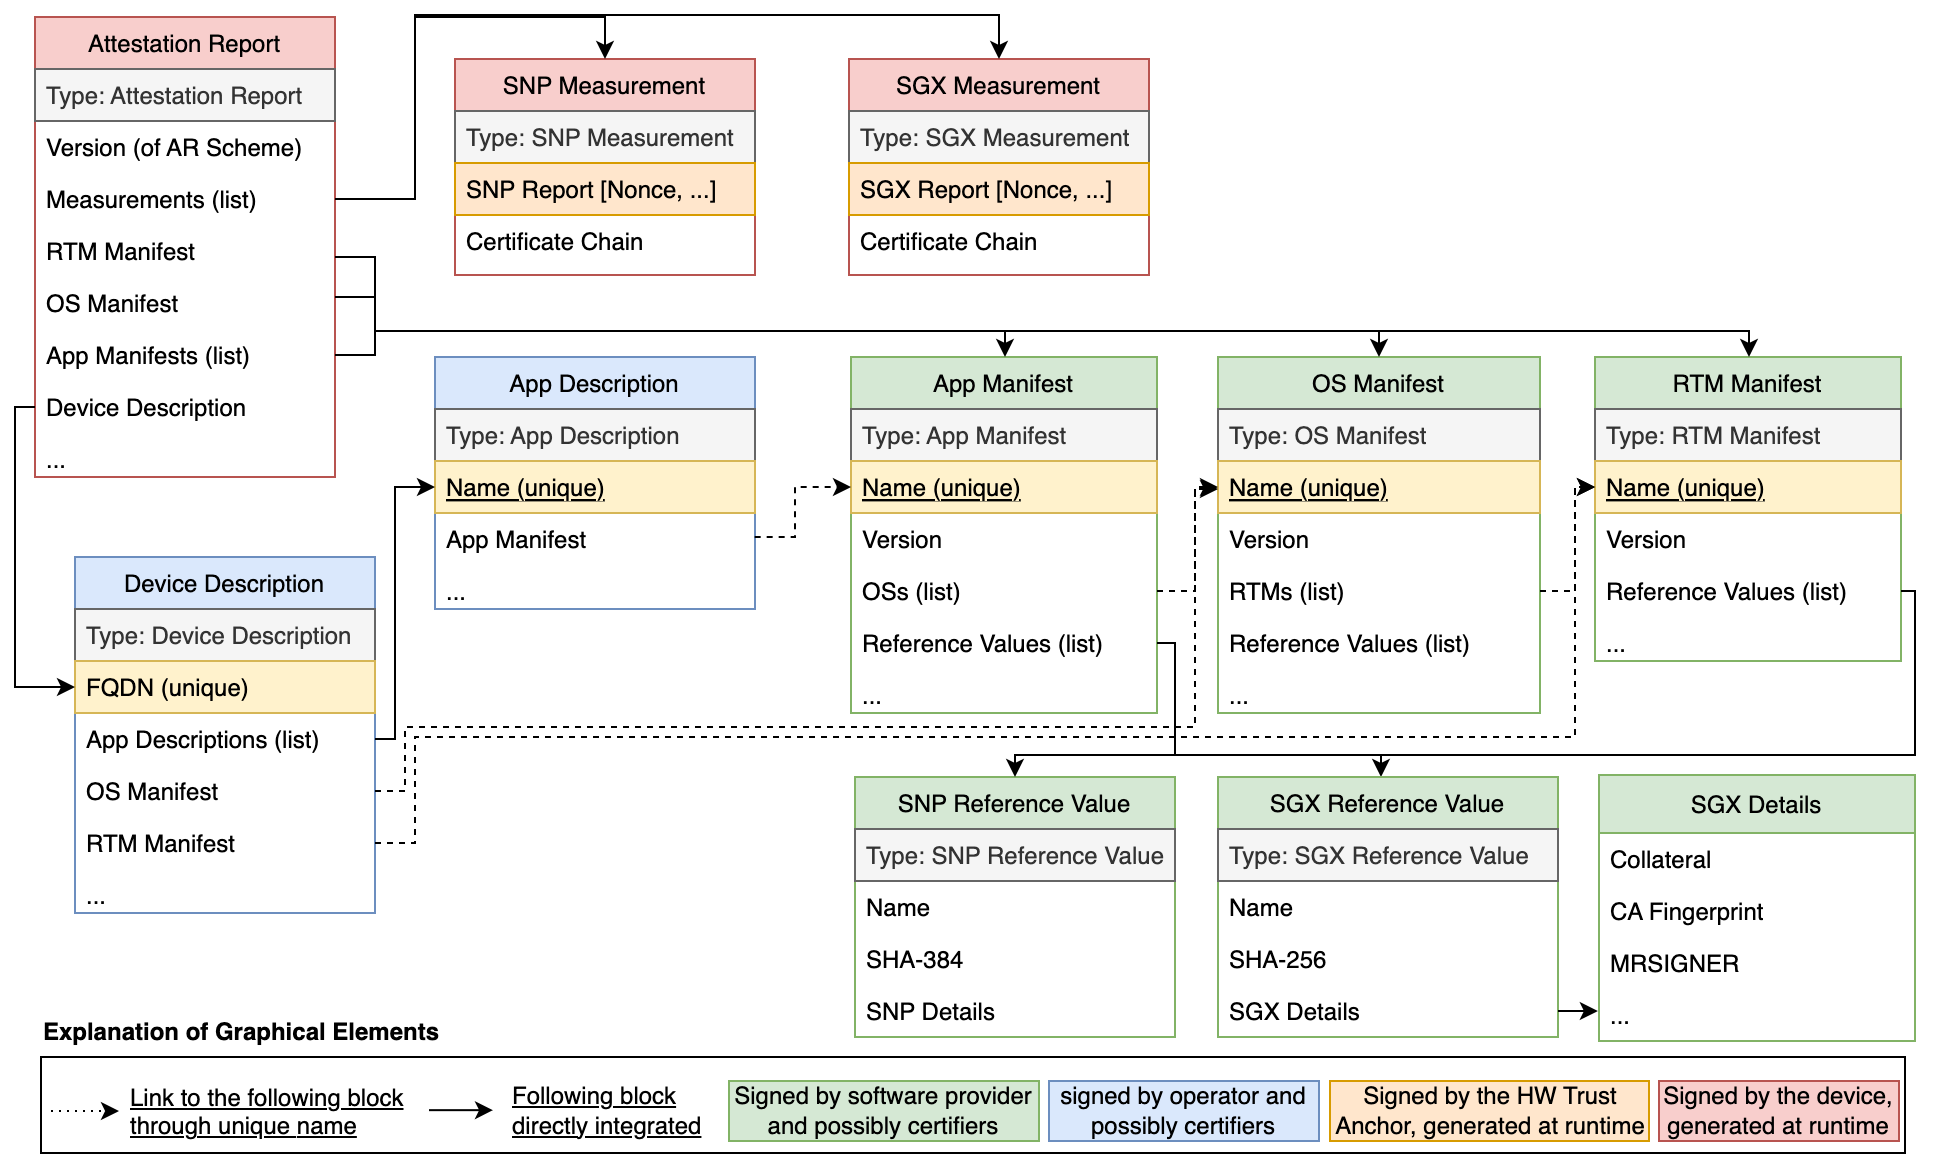
\includegraphics[width=1.0\linewidth]{figures/attestation_report.drawio.png}
	\end{center}
	\caption{CMC attestation report structure \cite{CMC_paper}} 
	\label{attestation-report}
\end{figure}

The architectural principle of the CMC framework demands that all data requried for the validation process is provided by the prover. A CMC report therefore encompasses three main elements: a list of measurements, a set of signed manifests containing platform, operating system, and software manifests, and a device description (see figure \ref{attestation-report}). The measurements can come from different sources, e.g. a SNP VM, a TPM, and are composed of attributes, such as a type, report, certificate chain, and optional parameters like hash chains.
Becuase every technology has a separate Measurement structure, such a data structure has to be implemented for the support of Intel SGX. Analogous to SNP measurements, SGX measurements comprise the same three fundamental elements: type, report, and certificate chain.

Reference Values about the platform, operating system and the software stack are included in signed manifest files (RTM, OS and app manifests) and linked together inside the device description of the attestation report (see figure \ref{attestation-report}). These manifests are typically created by the TEE owner and can be signed using the cmc signing tool. Following the design of SNP Reference Values, SGX Reference Values consist of a hash of the enclave pages (MRENCLAVE), which is typically published by the enclave developer and a SGX Details structure, comprising quote collateral, fingerprints/ hashes, a custom policy and other values for the verification process. Appart from the manifest, the device description also includes a Fully Qualified Domain Name (FQDN) to uniquely identify the platform. 

An important aspect of manifests is their temporal limited validity. By design RTM manifests as well as OS manifests are valid for a long period of time. Software on the other hand, is updated much more frequently and therefore software manifests have to be updated regularly. Depending on the concrete software, that is used inside the TEE, the validity period of software manifests can be restricted accordingly, e.g. to one or two days. For SGX however, software manifests are not an issue, because an enclave cannot execute multiple software, like a VM. Therefore only RTM and OS manifests are necessary. 

Another relvant aspect for SGX are CRLs. The Intel Root CA CRL is updated every year, the PCK CRL on the other hand every month. Consequently, the RTM manifests would also need to be updated regularly. This can be mitigated by shifting the acquisition of CRLs to the verifier side. 
Although this contradicts the principles of the cmc to a certain extent, since the verifier now has to make external queries to the PCS to retrieve necessary data for the report validation, the advantages make this acceptable. Replay attacks on the CRLs can be mitigated, since the verifier is trusted, and because the CRLs do not change often, it is sufficient if they are cached and only queried once a day. Hence there is virtually no overhead.
During the validation process, the CMC collects individual results and combines them inside a validation report, which is especially useful for debugging.\\
